\section{Results}
\label{sec:results}
As mentioned in Introduction, this section covers needed elements for understanding obtained results. We first describe our image dataset, and then we present produced results with the three methods.\par
\subsection{Dataset}
\label{sec:resulst:dataset}
All the data used in this study was provided by dermatology service of Saint Etienne hospital under patient consent. These data contain three types of images: Clinical Photography, Dermatoscopy and \ac{rcm}. Each of these modalities was acquired by a specialist. Furthermore, each patient is associated to a ground truth from histopathology \cite{Cinotti2018}.\par
We will focus only on the \ac{rcm} dataset. Images from this modality are acquired in the dermoepidermal junction, determined as relevant by specialist for diagnosis of Benign Lentigo and Malignant Lentigo. Images from this dataset have spatial resolution of 1000 by 1000 pixels, with a quantification on a single channel on 8 bits (0-255 grey levels).\par
As we want to learn from each individual image, a sub dataset has been built with help of dermatologist. A total of 70 patients \ac{rcm} images has been annotated, for an amount of 2100 \ac{rcm} images. Three types of labels have been assigned: "Malignant" label for images including at least malignant information, "Benign" label for images being composed of benign pathology and finally a "Healthy" label corresponding to absence of Malignant and Benign characteristics.\par
For convenience and for this particular work, we built with dermatologist a subset of this \ac{rcm} dataset, because native \ac{rcm} images can contain different kind of labels. These new data consist of small patches with a spatial resolution of 250 by 250 pixels. Each of these patches focus on its particular label. 200 images are extracted with the three labels mentioned previously. Fig. \ {fig:data} will gives an overview of such patches, which we want to classify.\par
\begin{figure}[h]
\centering
    \includegraphics[width=\linewidth]{content/figures/Data.png}
    \caption{Examples of extracted patches from skin dermal-epidermal junction with \ac{rcm}.}
    \label{fig:data}
\end{figure}
\subsection{Classification and Analysis}
\label{sec:result:classification}
Our validation protocol is equivalent for each experiment. For this purpose, a nested cross validation was used, as it’s known to be more unbiased and robust than simple cross validation schemes \cite{Cawley2010}. This process allows to cross validate hyperparameters of our network, and then evaluate more objectively our built models. Each of the cross-validation steps is based on K-Fold strategy of 5 folds. We make use of "Scikit Learn" library for Machine Learning classification, validation and metrics evaluation~\cite{pedregosa2011scikit}.\par
We evaluate our experiments using the following metrics: Precision, Recall and F1-Score. A standard deviation is calculated on each metric, to achieve an analysis of the stability of models along nested cross validation. Moreover, we extract \ac{roc} curves and Area Under Curve based on prediction probabilities, giving a better overview of sensibility/specificity compromises.\par
\begin{table}[h]
\centering
    \begin{tabular*}{0.45\textwidth}{l@{\extracolsep{\fill}}lll}
        \hline
        Methods & Precision & Recall & F1-Score \\
        \hline
        Wavelets & 0.69$\pm$0.04 & 0.69$\pm$0.04 & 0.68$\pm$0.05 \\
        \hline
        Haralick & 0.84$\pm$0.02 & 0.83$\pm$0.02 & 0.83$\pm$0.02 \\
        \hline
        Deep Learning & 0.89$\pm$0.02 & 0.89$\pm$0.02 & 0.89$\pm$0.02 \\
        \hline
    \end{tabular*}
    \caption{Patch classification average scores over the three exposed methods. Standard deviation is compute using outer cross validation.}
    \label{table:averages}
\end{table}
\Cref{table:averages} shows the obtained scores, for the three evaluated methods based on three metrics Precision, Recall and F1-Score. We observe a significant gap between Wavelets method, and Haralick / Deep Learning approaches. Also, computed standard deviation is more stable for Haralick and Deep Learning features, implying a more robust and reproducible scheme than for Wavelets. These results are correlated with observations made with a \ac{pca} projection along two first components, see \Cref{fig:projection}. Scatter graphs in Haralick and Deep Learning are more separable than for Wavelets.\par
\begin{figure}[h]
\centering
    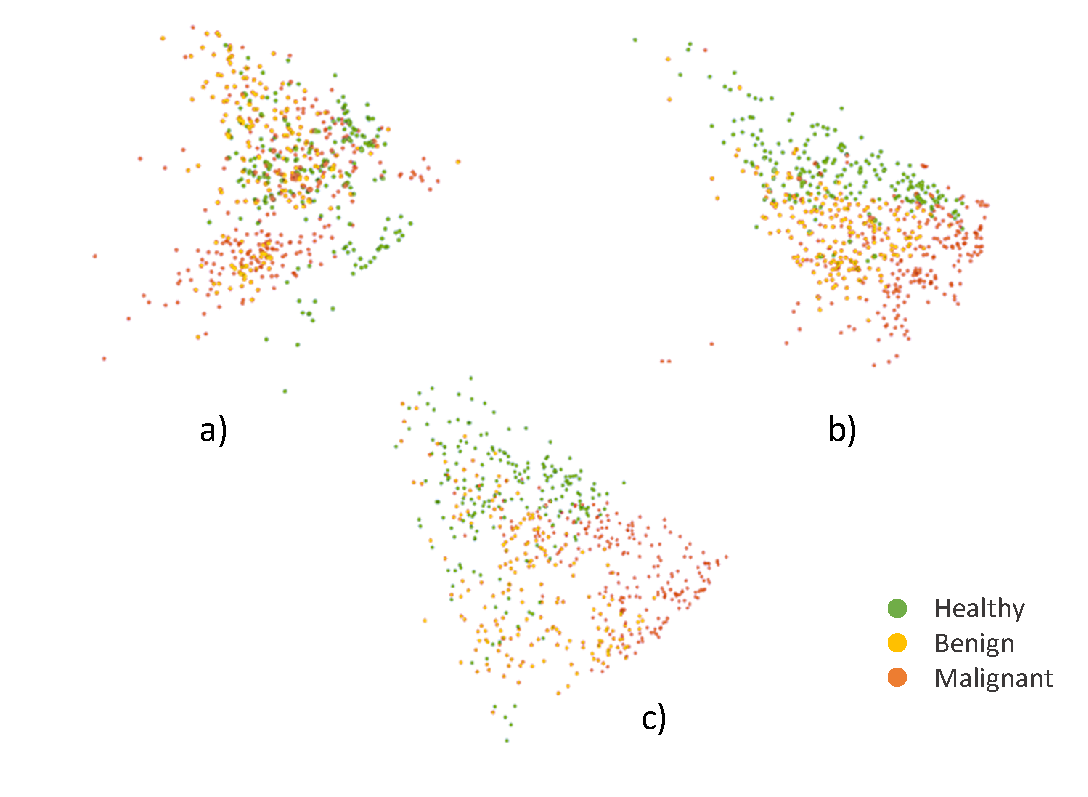
\includegraphics[width=\linewidth]{content/figures/Projection.pdf}
    \caption{Feature representation along two first \ac{pca} components. From a) to c): Wavelets, Haralick and Deep features extraction.}
    \label{fig:projection}
\end{figure}
An in-depth analysis of Deep Learning scores provides more information on achieved classification is shown in \Cref{table:deep_scores}. Classification of "Healthy" skin seems more efficient and more robust than others. This phenomenon is also visible on extracted \ac{roc} curves in \Cref{fig:roc}. This behavior could be expected as we divide Lentigo pathology in two sub categories. Images in these categories have a multitude of similar patterns, and are more difficult to distinguish.\par
\begin{table}[h]
\centering
    \begin{tabular*}{0.45\textwidth}{l@{\extracolsep{\fill}}lll}
        \hline
        Labels & Precision & Recall & F1-Score \\
        \hline
        Healthy & 0.96$\pm$0.03 & 0.95$\pm$0.02 & 0.96$\pm$0.02 \\
        \hline
        Benign & 0.86$\pm$0.04 & 0.88$\pm$0.06 & 0.87$\pm$0.04 \\
        \hline
        Malignant & 0.84$\pm$0.05 & 0.83$\pm$0.01 & 0.84$\pm$0.03 \\
        \hline
        Average & 0.89$\pm$0.02 & 0.89$\pm$0.02 & 0.89$\pm$0.02 \\
        \hline
    \end{tabular*}
    \caption{Patch classification scores on Deep Learning.}
    \label{table:deep_scores}
\end{table}
\begin{figure}[h]
\centering
    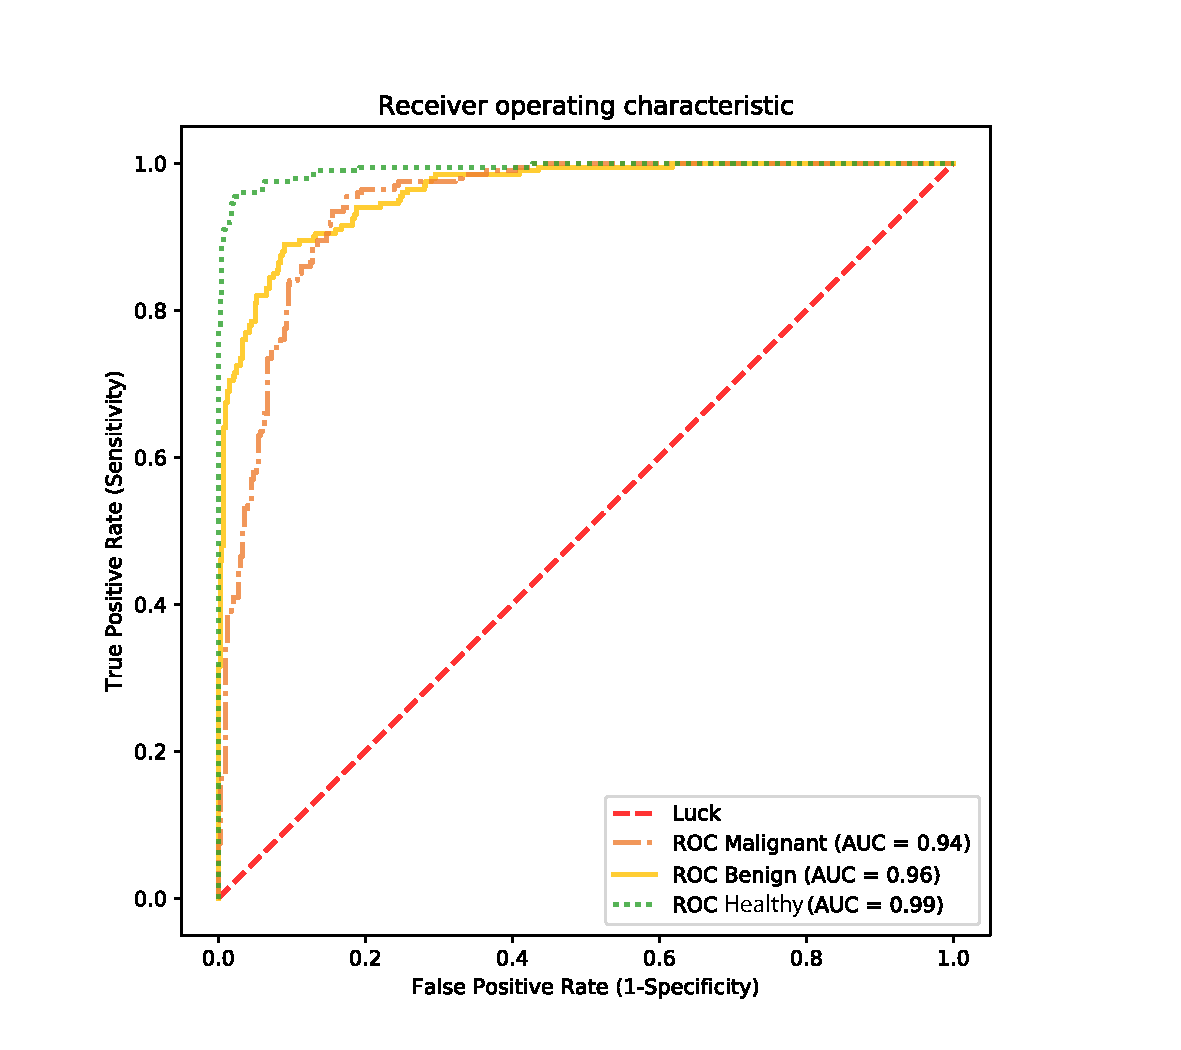
\includegraphics[width=\linewidth]{content/figures/ROC.pdf}
    \caption{Extracted \ac{roc} curves in deep features classification, for Healthy, Benign and Malignant.}
    \label{fig:roc}
\end{figure}